\documentclass{standalone}
\usepackage{tikz}
\usepackage{circuitikz}
\usetikzlibrary{positioning}

\begin{document}
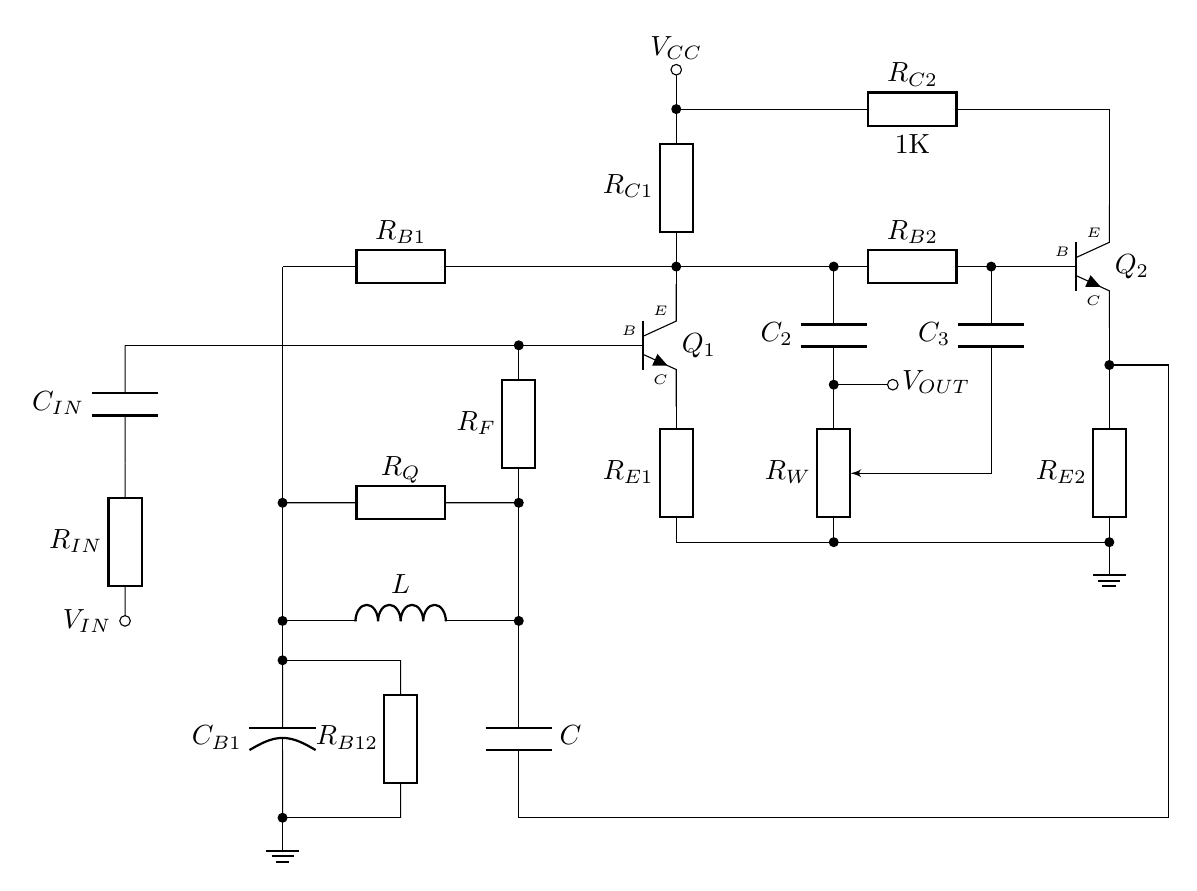
\begin{tikzpicture}	
	\draw (1, 3.5) to[european resistor, l=$R_{IN}$] (1, 5.5);
	\draw (6, 8) to[european resistor, l_=$R_{B1}$] (3, 8);
	\draw (4.5, 3) to[european resistor, l_=$R_{B12}$] (4.5, 1);
	\draw (12, 8) to[european resistor, l_=$R_{B2}$] (10, 8);
	\draw (8, 8) to[european resistor, l=$R_{C1}$] (8, 10);
	\draw (13.5, 10) to[european resistor, l_=$R_{C2}$] (8.5, 10);
	\draw (8, 4.5) to[european resistor, l=$R_{E1}$] (8, 6.25);
	\draw (13.5, 4.5) to[european resistor, l=$R_{E2}$] (13.5, 6.25);
	\draw (6, 5) to[european resistor, l=$R_F$] (6, 7);
	\draw (6, 5) to[european resistor, l_=$R_Q$] (3, 5);

	\draw (10, 6.25) to[european potentiometer, l_=$R_W$] (10, 4.5);

	\draw (1, 5.5) to[capacitor, l=$C_{IN}$] (1, 7);
	\draw (10, 6.25) to[capacitor, l=$C_2$] (10, 8);
	\draw (12, 6.25) to[capacitor, l=$C_3$] (12, 8);
	\draw (3, 3) to[curved capacitor, l_=$C_{B1}$] (3, 1);
	\draw (6, 1) to[capacitor, l_=$C$] (6, 3);

	\draw (3, 3.5) to[american inductor, l=$L$] (6, 3.5);

	\node[npn] at (13.5, 8) {$Q_2$};
	\node[npn] at (8, 7) {$Q_1$};

	\draw (7.16, 7) -- (1, 7);	
	\draw (4.5, 3) -- (3, 3);
	\draw (4.5, 1) -- (3, 1);
	\draw (3, 3) -- (3, 8);
	\draw (6, 3) -- (6, 5);
	\draw (6, 8) -- (10, 8);
	\draw (6, 1) -- (14.25, 1) -- (14.25, 6.75) -- (13.5, 6.75);
	\draw (8, 4.5) -- (13.5, 4.5);
	\draw (8, 10) -- (8.5, 10);
	\draw (8, 10) -- (8, 10.5);
	\draw (8, 7.75) -- (8, 8);
	\draw (10, 6.5) -- (10.75, 6.5);
	\draw (10.56, 5.375) -| (12, 6.25);
	\draw (12, 8) -- (12.66, 8);
	\draw (13.5, 8.77) -| (13.5, 10);
	\draw (13.5, 7.23) -- (13.5, 6.25);

	\node[ground] at (13.5, 4.5) {};
	\node[ground] at (3, 1) {};
	\node[circ] at (10, 4.5) {};
	\node[circ] at (10, 8) {};
	\node[circ] at (12, 8) {};
	\node[circ] at (13.5, 4.5) {};
	\node[circ] at (13.5, 6.75) {};
	\node[circ] at (3, 1) {};
	\node[circ] at (3, 3) {};
	\node[circ] at (3, 3.5) {};
	\node[circ] at (3, 5) {};
	\node[circ] at (6, 3.5) {};
	\node[circ] at (6, 5) {};
	\node[circ] at (6, 7) {};
	\node[circ] at (8, 10) {};
	\node[circ] at (8, 8) {};
	\node[circ] at (10, 6.5) {};
	\node[ocirc, scale=1.2] at (10.75, 6.5) {};
	\node[ocirc, scale=1.2] at (8, 10.5) {};
	\node[ocirc, scale=1.2] at (1, 3.5) {};
	\node[below=0.2cm of {11, 10}] {1K};
	\node[above=0cm of {8, 10.5}] {$V_{CC}$};
	\node[left=0.05cm of {1, 3.5}] {$V_{IN}$};
	\node[below=-0.3cm of {11.3, 6.5}] {$V_{OUT}$};
	\node[font=\tiny, above=0.0cm of {(12.9,8)}] {$B$};
	\node[font=\tiny, above=0.0cm of {(7.4,7)}] {$B$};
	\node[font=\tiny, above=0.25cm of {(13.3,8)}] {$E$};	
	\node[font=\tiny, above=0.25cm of {(7.8,7)}] {$E$};	
	\node[font=\tiny, below=0.25cm of {(13.3,8)}] {$C$};
	\node[font=\tiny, below=0.25cm of {(7.8,7)}] {$C$};

\end{tikzpicture}
\end{document}